In this kind of survey, it is essential to ensure the participants’ diversity to get sufficiently accurate and generally reflective results. The Android developer survey found participants in 5 different countries (Germany, Turkey, Portugal, Estonia and, Russia) through the author's current and former colleagues. The survey was answered by Android developers working in 7 different well-known companies in these countries. Also, as previously stated in the 3rd part, the survey reached answers from random Android developers through various social media platforms. In this way, the participants’ diversity was increased, and getting better results was ensured. 

Also, the first question was added to the survey to learn about the competence of participants. As can be guessed, the probability of getting more accurate results from a survey formed to determine the preferred technology and methods for Android application development is directly proportional to the participants’ experience. Results can be seen in Fig. \ref{fig:participant_bg} below.
\begin{figure}[ht!]
    \centering
    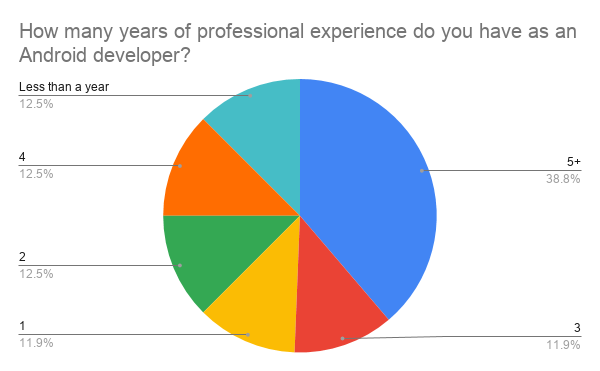
\includegraphics[scale=0.25]{figures/survey_q1_dev_experience.png}
    \caption{Participant background results}
    \label{fig:participant_bg}
\end{figure}
\FloatBarrier

As stated before, the participant diversity was provided to improve the accuracy of the survey. When the chart above is examined, 63\% of the participants have more than three years of experience while 40\% of them has 5+ years of experience. People with 0-2 years of experience are around 37\% of the all participants.